\documentclass[a4paper,10pt]{article}
\usepackage[utf8]{inputenc}
\usepackage{url}
\usepackage{amsmath}
\usepackage{graphicx}

%opening
\title{COMP417: Assignment 3\\Due Friday, March 24  at 6pm}
\author{}

\begin{document}

\maketitle


\section{Occupancy grid mapping (5pts)}
In this exercise you are going to implement parts of the occupancy grid mapping system discussed in class. In particular, you are going to map an environment 
based on known odometry estimates and known 2D laser scans. Do \path{git} $\;$ \path{pull} under your comp417 repository to get the starter code. The functionality 
that you need to implement is marked using to-do comments in the file \path{estimation_assignment/python/occupancy_grid_mapper.py}. To run your code, 
\path{cd} $\;$ \path{path/to/comp417/estimation_assignment/} and execute the following commands on three different terminals: 
\newline

  \path{rosbag} $\;$ \path{play} $\;$ \path{laser_and_odometry.bag}
  
  \path{roslaunch} $\;$ \path{estimation_assignment} $\;$ \path{occupancy_grid_mapping.launch} $\;$ \path{odometry_orientation_noise_std_dev:=2.5} $\;$ \path{odometry_position_noise_std_dev:=0.1}
  
  \path{rosrun} $\;$ \path{rviz} $\;$ \path{rviz} 
\newline
\newline
\noindent When rviz initializes, go to \path{File} $>$ \path{Open Config} and then load the configuration file in \path{estimation_assignment/resources/comp417.rviz}
which is going to start the visualization of laser scan messages, frames of reference, and debugging visualizations. Save this configuration file as the default
in your \path{/home/username/.rviz/default.rviz}, so you won't have to do this every time you restart rviz. In the \path{roslaunch} command given above, the standard deviation of 
the odometry orientation noise is given in degrees. In this example the true yaw of the robot is corrupted by random noise from $\mathcal{N}(0, 2.5^2)$. Similarly, the true position 
is corrupted by random noise from $\mathcal{N}(0, 0.1^2)$, which is expressed in meters. \path{laser_and_odometry.bag} is a recording of laser scans and odometry data in the environment 
you used in Assignment 1. The expected result for perfect odometry looks similar to Figure \ref{fig:gmapping}. 
\newline
\newline
\newline
\noindent What you need to submit: 5 images of maps produced by your mapper, with noise parameters (0, 0), (2.5, 0), (5, 0), (2.5, 0.1), (5, 0.1) respectively. 
Your images should be named \path{map_[0|1|2|3|4]_firstname_lastname.png}. Also, submit a video recording of the rviz visualization for the odometry noise combination (0,0),
demonstrating your map being built from beginning to end. Your video should be named \path{map_0_firstname_lastname.mp4/avi/ogg}. 

\section{Depth from stereo disparity (6.25pts)}
In this exercise you are going to solve the depth from stereo disparity problem that we discussed in class. You will be given pairs of stereo-rectified images from the 
KITTI and Middlebury datasets, such as the ones outlined in Fig.~\ref{fig:kitti_stereo}. The KITTI dataset is currently the state-of-the-art benchmarking service for various 
visual tasks that are relevant to self-driving cars. Its data is taken from a car equipped with the same sensors as most self-driving cars\footnote{\url{http://www.cvlibs.net/datasets/kitti/setup.php}}.
The Middlebury dataset\footnote{\url{http://vision.middlebury.edu/stereo/data/scenes2014/}} is one of the oldest computer vision benchmarking services out there, and has become
very popular for its stereo evaluation suite. You are encouraged to explore these datasets to become aware of what they offer. In the meantime, we are going to use the following rectified stereo 
image pairs for this assignment:
\begin{figure}[h!]
  \begin{center}
    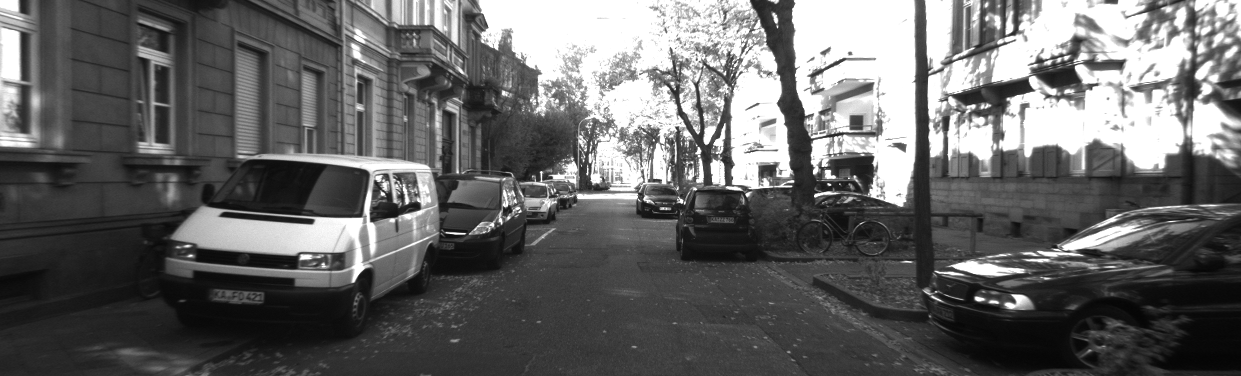
\includegraphics[width=0.45\textwidth]{stereo_images/images0/kitti_1_left}
    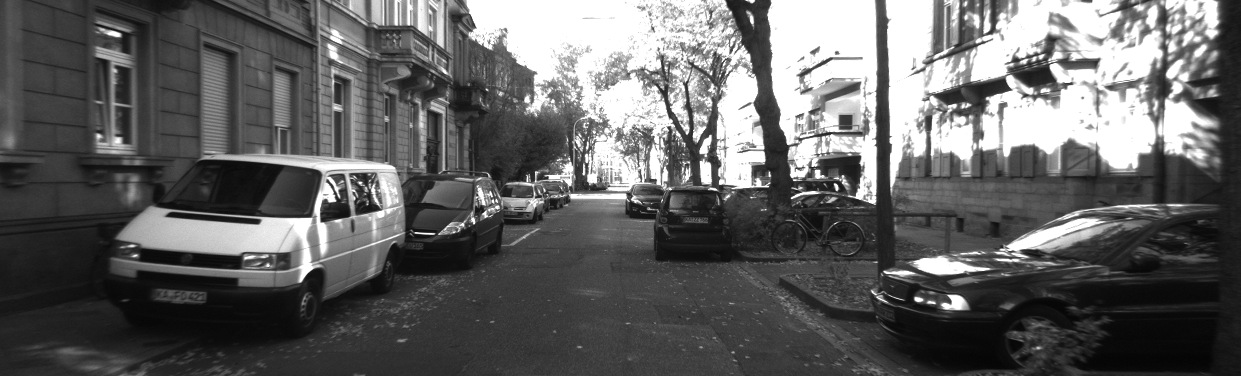
\includegraphics[width=0.45\textwidth]{stereo_images/images1/kitti_1_right}
  \end{center}
\end{figure}  

\begin{figure}[h!]
  \begin{center}  
    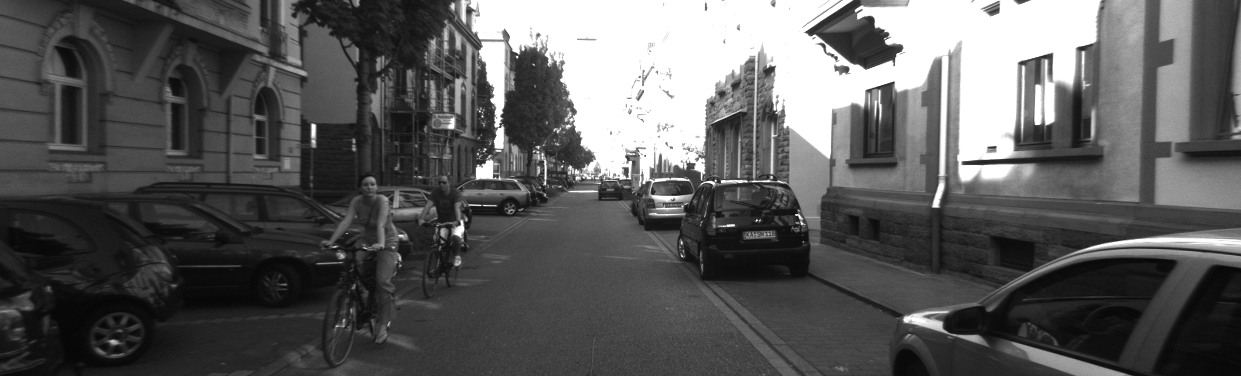
\includegraphics[width=0.45\textwidth]{stereo_images/images0/kitti_2_left}
    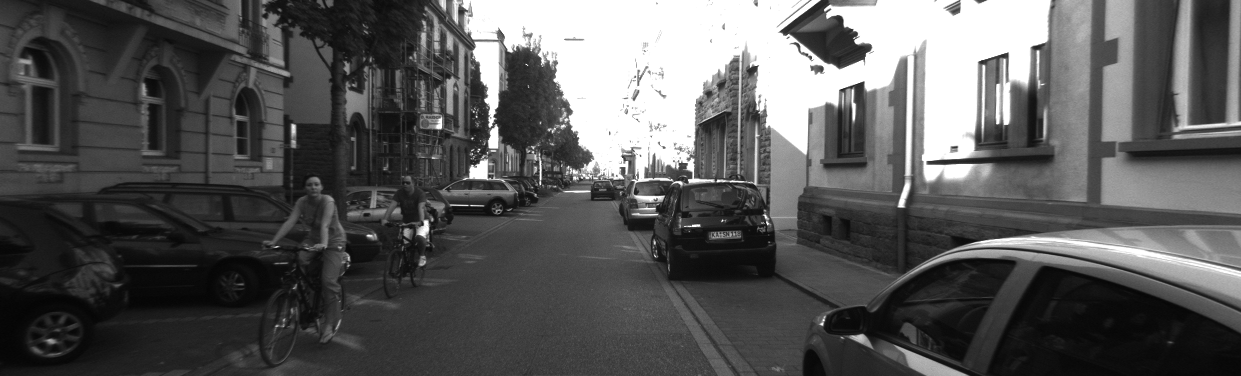
\includegraphics[width=0.45\textwidth]{stereo_images/images1/kitti_2_right}
\end{center}
\end{figure}  
    
\begin{figure}[h!]
  \begin{center}     
    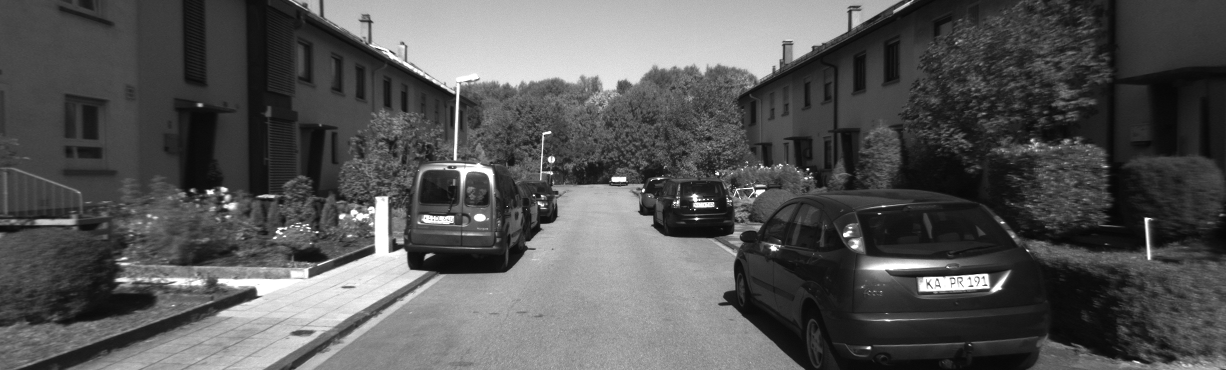
\includegraphics[width=0.45\textwidth]{stereo_images/images0/kitti_3_left}
    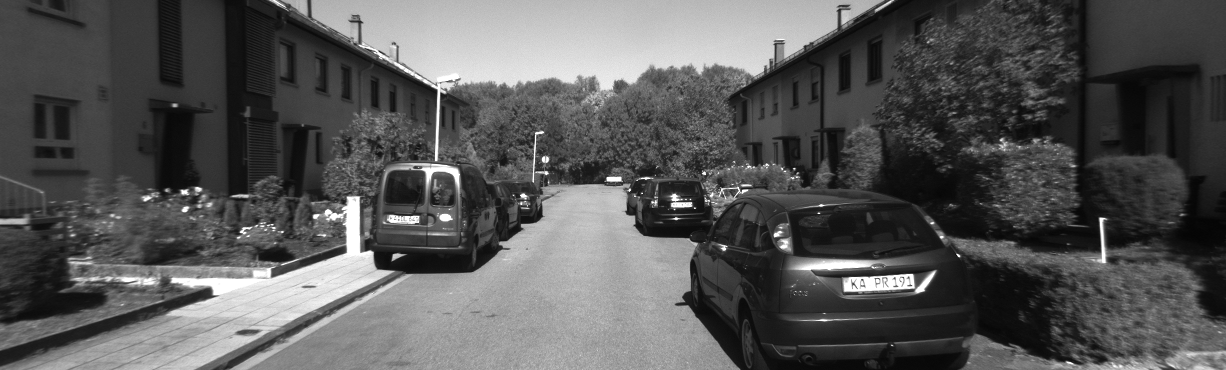
\includegraphics[width=0.45\textwidth]{stereo_images/images1/kitti_3_right}
\end{center}
\end{figure}  

\begin{figure}[h!]
  \begin{center}         
    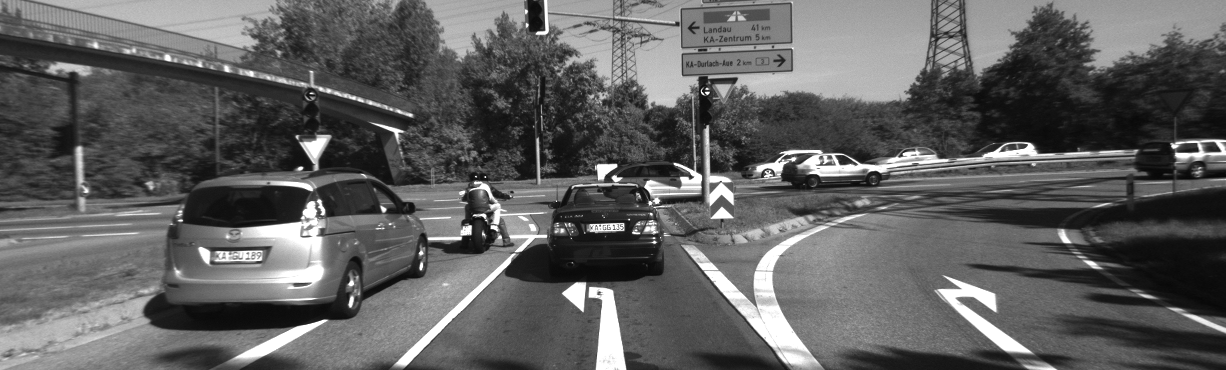
\includegraphics[width=0.45\textwidth]{stereo_images/images0/kitti_4_left}
    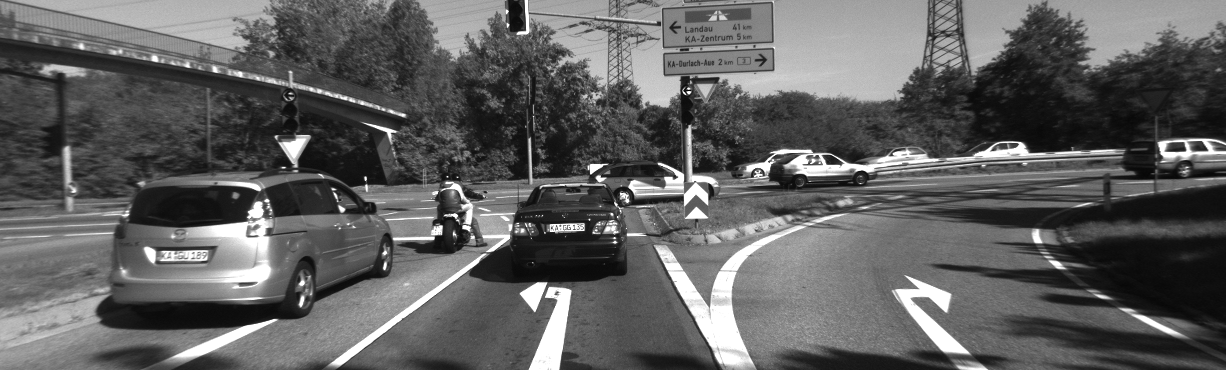
\includegraphics[width=0.45\textwidth]{stereo_images/images1/kitti_4_right}
\end{center}
\end{figure}  
    
 \begin{figure}[h!]
  \begin{center}  
    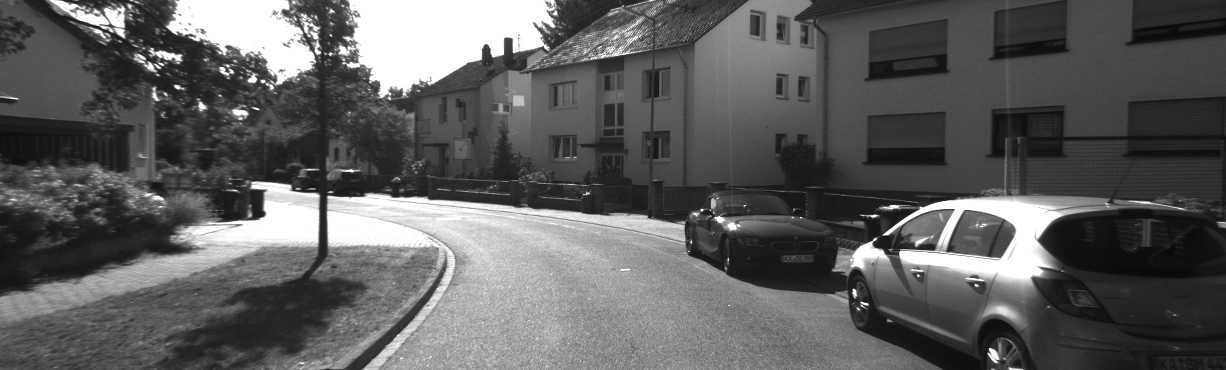
\includegraphics[width=0.45\textwidth]{stereo_images/images0/kitti_5_left}
    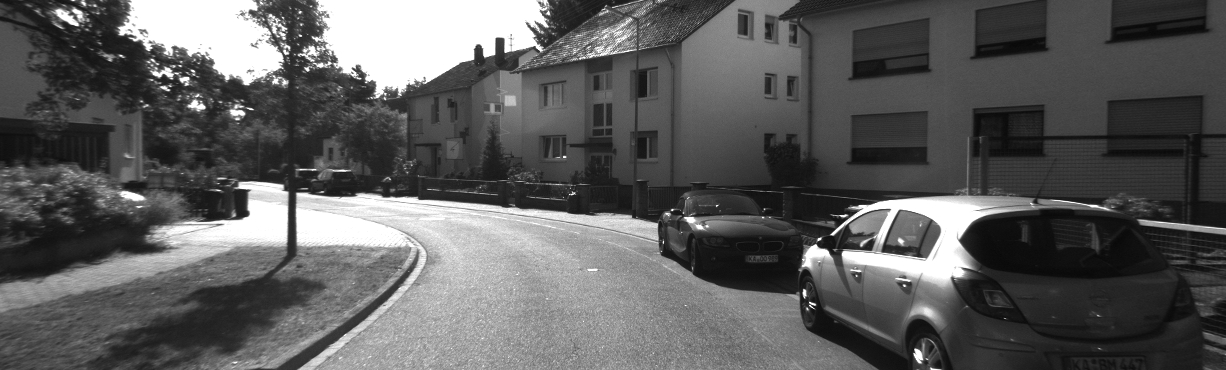
\includegraphics[width=0.45\textwidth]{stereo_images/images1/kitti_5_right}
\end{center}
\end{figure}  

    
\begin{figure}[h!]
  \begin{center}  
    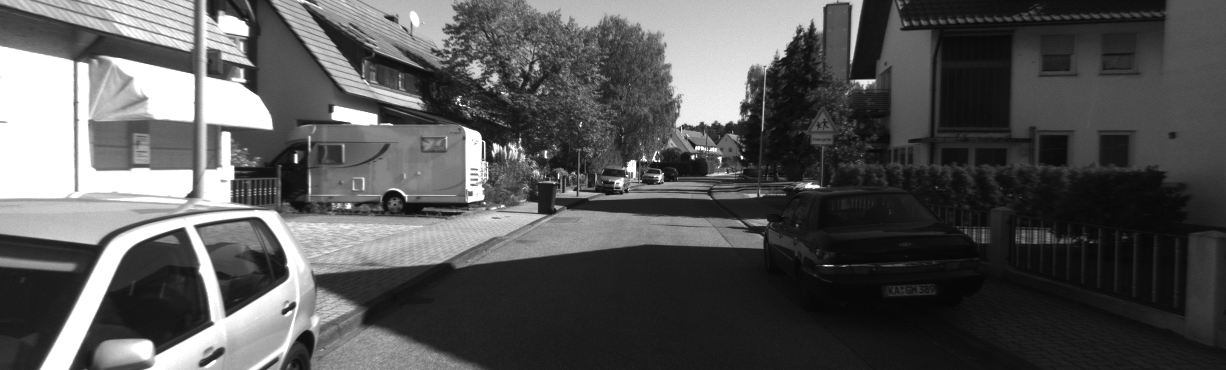
\includegraphics[width=0.45\textwidth]{stereo_images/images0/kitti_6_left}
    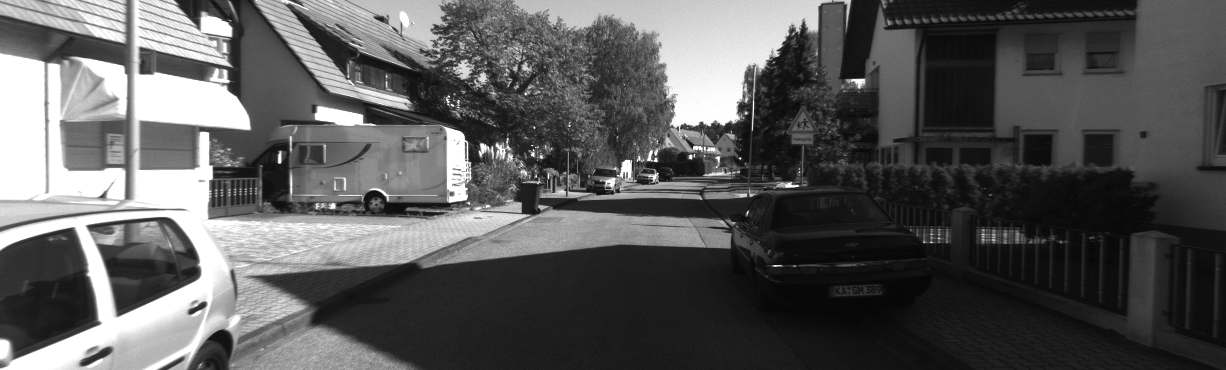
\includegraphics[width=0.45\textwidth]{stereo_images/images1/kitti_6_right}
\end{center}
\end{figure}  
    
    
\begin{figure}[h!]
  \begin{center}    
    \includegraphics[width=0.35\textwidth]{stereo_images/images0/middlebury_1_left}
    \includegraphics[width=0.35\textwidth]{stereo_images/images1/middlebury_1_right}
  \end{center} 
  \caption{Stereo image pairs 1 to 6 are from the KITTI dataset. The baseline between the cameras is about 0.5 meters. The 7th image pair is from the Middlebury stereo dataset. The baseline is about 0.2 meters.}
  \label{fig:kitti_stereo}
\end{figure}
\noindent For each of these image pairs you will compute the disparity map in pixels, using block matching along horizontal epipolar lines, as we saw in class. Note that this is definitely not the state-of-the-art
algorithm for stereo disparity, and your implementation will most likely not run in real-time, but it is enough to get you thinking about the problem. 
\newline
\newline
\noindent Given the stereo camera calibration and rectification parameters 
you will compute the depth map in metric coordinates from the pixel disparity map. For example, these disparity maps have been obtained with patches of width 64 pixels, and the sum of squared differences as the distance 
metric for matching patches along the horizontal epipolar lines. The most common options for a distance metric for comparing similarity between image patches are:
\begin{itemize}
 \item sum of absolute differences (SAD), $\sum_{i,j}|L_{ij} - R_{ij}|$, where L,R are the left and right patches being examined.
 \item sum of squared differences (SSD), $\sum_{i,j}(L_{ij} - R_{ij})^2$
 \item normalized cross-correlation (NCC), $\sum_{i,j} \frac{(L_{ij} - \mu_L)}{\sqrt{\sum_{ij}{L_{ij} - \mu_L}}} \frac{(R_{ij} - \mu_R)}{\sqrt{\sum_{ij}{R_{ij} - \mu_R}}}$
\end{itemize}
\noindent The expected results you should get look approximately like this: 
\begin{figure}[h!]
  \begin{center}
    \includegraphics[width=0.45\textwidth]{results/kitti_1_disparity}
    \includegraphics[width=0.45\textwidth]{results/kitti_1_depth}
   \end{center}
\end{figure}
    
\begin{figure}[h!]
  \begin{center}
    \includegraphics[width=0.45\textwidth]{results/kitti_2_disparity}
    \includegraphics[width=0.45\textwidth]{results/kitti_2_depth}
   \end{center}
\end{figure}

\begin{figure}[h!]
  \begin{center}
    \includegraphics[width=0.45\textwidth]{results/kitti_3_disparity}
    \includegraphics[width=0.45\textwidth]{results/kitti_3_depth}
   \end{center}
\end{figure}

\begin{figure}[h!]
  \begin{center}
    \includegraphics[width=0.45\textwidth]{results/kitti_4_disparity}
    \includegraphics[width=0.45\textwidth]{results/kitti_4_depth}
   \end{center}
\end{figure}

\begin{figure}[h!]
  \begin{center}
    \includegraphics[width=0.45\textwidth]{results/kitti_5_disparity}
    \includegraphics[width=0.45\textwidth]{results/kitti_5_depth}
   \end{center}
\end{figure}

\begin{figure}[h!]
  \begin{center}
    \includegraphics[width=0.45\textwidth]{results/kitti_6_disparity}
    \includegraphics[width=0.45\textwidth]{results/kitti_6_depth}
   \end{center}
\end{figure}

\begin{figure}[h!]
  \begin{center}
    \includegraphics[width=0.45\textwidth]{results/middlebury_1_disparity}
    \includegraphics[width=0.45\textwidth]{results/middlebury_1_depth}
  \end{center} 
  \caption{Example disparity and depth maps for the image pairs presented above. No post-processing has been applied to the disparity maps to encourage smoothness.}
  \label{fig:results}
\end{figure}
\subsubsection{Starter code}
\noindent You are given starter code in your comp417 repository under \path{estimation_and_vision_assignment/python/stereo_disparity_map.py}. The way to run this code is:
\newline
\newline
\path{./stereo_disparity_map.py} $\;$ \path{../latex/stereo_images/images0/kitti_1_left.png} $\;$ \path{../latex/stereo_images/images1/kitti_1_right.png} $\;$ \path{../resources/kitti.yaml}
\newline
\newline
\noindent and similarly for the motorbike photo:
\path{./stereo_disparity_map.py} $\;$ \path{../latex/stereo_images/images0/middlebury_1_left.png} $\;$ \path{../latex/stereo_images/images1/middlebury_1_right.png} $\;$ \path{../resources/middlebury.yaml}
\newline
\newline
\noindent The \path{.yaml} files contain rectification parameters and other parameters for the two datasets.
\subsubsection{What to submit}
Your implementation of disparity and depth estimation in \path{estimation_and_vision_assignment/python/stereo_disparity_map.py} using sum of squared differences for matching. Also, the following 14 images: 
7 disparity maps and 7 depth maps for each of the image pairs mentioned above. Your files should be named \path{kitti_[1-6]_disparity.png}, \path{kitti_[1-6]_depth.png}, \path{middlebury_1_disparity.png}, \path{middlebury_1_depth.png}

\subsection{Bonus (2 pts)}
Try to use GPU acceleration to make your stereo block matching code run closer to real-time. For the size of these image pairs for example, it could be made to run closer to 1 sec
with a good implementation and on a modern GPU. 


\section{How to submit}
Submit all your work in a file called \path{estimation_assignment.zip} that contains your extensions to the provided starter code, as well as the five images, the video, and the pdf file. 
Submissions will be done on myCourses. 

\section{A note on indentation}
Please make sure your editor uses spaces instead of tab characters, otherwise your TAs will have a hard time reading your code on their editors, which might be different from yours.
\end{document}
